%% LyX 2.3.7 created this file.  For more info, see http://www.lyx.org/.
%% Do not edit unless you really know what you are doing.
\documentclass[english]{article}
\usepackage[T1]{fontenc}
\usepackage[latin9]{inputenc}
\usepackage{url}
\usepackage{graphicx}
\usepackage{esint}

\makeatletter

%%%%%%%%%%%%%%%%%%%%%%%%%%%%%% LyX specific LaTeX commands.
%% Because html converters don't know tabularnewline
\providecommand{\tabularnewline}{\\}

\makeatother

\usepackage{babel}
\begin{document}
\title{Solving differential equations with global optimization techniques}
\author{Ioannis G. Tsoulos$^{(1)}$\thanks{Corresponding author. Email: itsoulos@uoi.gr},
Alexandros Tzallas$^{(1)}$, Dimitrios Tsalikakis$^{(2)}$}
\date{$^{(1)}$Department of Informatics and Telecommunications, University
of Ioannina, 47100 Arta, Greece \\
$^{(2)}$University of Western Macedonia, Department of Engineering
Informatics and Telecommunications, Greece\\
}
\maketitle
\begin{abstract}
The solution of differential equations finds many applications in
a huge range of problems, and many techniques have been developed
to approximate their solutions. For example, differential equations
can be applied to physics problems, chemistry problems, economics,
modeling etc. This manuscript presents a number of global optimization
techniques that have been successfully applied to train machine learning
models to approximate differential equation solutions. More specifically,
two modified versions of genetic algorithms and particle swarm optimization
methods are proposed here. These methods have been successfully applied
to solving ordinary differential equations and systems of differential
equations as well as partial differential equations with Dirichlet
boundary conditions.
\end{abstract}
\textbf{Keywords}: Differential equations; global optimization; stochastic
methods; machine learning

\section{Introduction}

The solution of ordinary differential equations (ODEs), systems of
differential equations (SODEs) and partial differential equations
(PDEs) is commonly used in many scientific fields, like physics \cite{de_physics1,de_physics2},
chemistry \cite{de_chem1,de_chem2,de_chem3}, economics \cite{de_econ1,de_econ2},
biology \cite{de_bio1,de_bio2} etc. It is obvious that the numerical
solution of differential equations has positive effects in many scientific
areas and, as a result, many techniques have been published in the
modern literature. These methods can include the well - known Runge
Kutta methods \cite{de_rk1,de_rk2,de_rk3}, wavelet transformations
\cite{de_wave1,de_wave2,de_wave3}, predictor - corrector variations
\cite{de_pred1,de_pred2}, methods that incorporate artificial neural
networks \cite{neural1,neural2} to solve differential equations \cite{de_nn1,de_nn2,de_nn3},
finite element methods \cite{de_finite1,de_finite2} etc. Similar,
semi - implicit composition methods have been proposed to solve differential
equations like the work of Chen and Shen, used to solve the Ginzburg---Landau
equation and the Cahn---Hilliard equation \cite{de_semimplicit1}.
Likewise, Fedoseev et al proposed a novel algorithm for Semi-Implicit
Composition ODE Solvers \cite{de_semiimplicit2}. Also, semi-explicit
composition methods have been proposed for the solution of differential
equations \cite{de_semiexplicit}. Similar, semi-implicit predictor--corrector
methods have been used for practical problems modeled as differential
equations \cite{de_semipred1,de_semipred2}. Recently, another technique
based on Grammatical Evolution \cite{ge_main} has been proposed to
tackle differential equations in closed analytical form by Tsoulos
and Lagaris \cite{de_tsoulos}. 

In this work, the differential equations to be solved are presented
as machine learning models and the solution of the corresponding equation
is reduced to a global optimization problem, where the task is to
locate the global minimum of a continuous and differentiable function
$f:S\rightarrow R,S\subset R^{n}$ and it is defined as: 
\begin{equation}
x^{*}=\mbox{arg}\min_{x\in S}f(x)\label{eq:eqOptimization}
\end{equation}
with $S$: 
\[
S=\left[L_{1},R_{1}\right]\otimes\left[L_{2},R_{2}\right]\otimes\ldots\left[L_{n},R_{n}\right]
\]
The value of $n$ is the number of parameters in the corresponding
machine learning model. For example, the number of weights and biases
in some artificial neural network. The vector $L$ is considered as
the left margin of the parameter $x$, and the vector $R$ as the
right margin. Machine learning models have been used a lot in solving
differential equations. For example, the use of SVM techniques \cite{de_svm1,de_svm2},
the incorporation of deep learning methods \cite{de_deep1,de_deep2},
constructed neural networks \cite{de_nnc} etc. In current work, two
machine learning models were tested: artificial neural networks and
Radial Basis Function networks (RBF) \cite{RbfMain}. The parameters
in these machine learning models were trained using modified versions
of two well-known global optimization techniques: Genetic Algorithms
\cite{ga1,ga2,ga3} and the PSO method \cite{pso1,pso2}. In the present
work, these two global optimization techniques were chosen as they
have been used in dozens of practical problems and are easily adaptable
to the problem. Furthermore, both methods can be easily parallelized
\cite{gen_par1,gen_par2,gen_par3}\textbf{ }to take advantage of modern
parallel architectures and are tolerant of numerical errors and noise
that may be present in the data. The proposed method has been successfully
used to solve ordinary differential equations, systems of differential
equations as well as partial differential equations with Dirichlet
boundary conditions.

In the proposed methodology, the problem of numerically solving differential
equations has been reduced to a machine learning model parameterization
problem using global optimization techniques. Consequently, any global
optimization method can be used to solve differential equations, even
techniques with parallelization capabilities, such as Genetic Algorithms
for example. This means that the proposed technique could also be
used to solve difficult problems of differential equations, such as
for example large systems of ordinary differential equations.

Recently , Effati et al \cite{nn_de_similar1} used artificial neural
networks for solving differential equations. Also, Pakdaman et al
\cite{nn_de_similar2} used artificial neural networks to solve differential
equations of fractional order. Furthermore, Admon et al proposed an
algorithm based on artificial neural networks for solving differential
equations of fractional order.

The rest of this article is organized as follows: in section \ref{sec:Method-description}
the used models and the proposed modified global optimization techniques
are outlined in detail. In section \ref{sec:Experiments} the differential
equations used in the experiments are listed as well as the experimental
results and, finally in section \ref{sec:Conclusions} some conclusions
about the used methods are presented.

\section{Method description \label{sec:Method-description}}

The proposed technique minimizes the error of machine learning models,
which are used as solvers of differential equations. Therefore, the
section starts with the definition of the error for each differential
equation case and continues with the definition of the machine learning
models used and ends with the global optimization techniques used
to minimize the error of the differential equations.

\subsection{Calculation of error for the machine learning models \label{subsec:Calculation-of-error}}

This subsection details the calculation of the errors of the machine
learning models for each differential equation. In each equation case,
the initial or boundary conditions are imposed using penalty factors.

\subsubsection{Calculation for ODEs }

An ordinary differential equation can be defined as: 
\begin{equation}
\psi\left(t,y,y^{(1)},\ldots,y^{(n)}\right)=0,\ t\in[a,b]
\end{equation}
where the quantity $y^{(i)}$ stands for the ith-order derivative
of $y(x).$ Also, the initial conditions for the equation are given
by: 
\begin{equation}
h_{i}\left(t_{i},y,y^{(1)},\ldots,y^{(n)}\right),i=1,\ldots,n
\end{equation}
where $t_{i}$ can be $a$ or $b$. The calculation of the model error
$f(r)$ of a given machine learning model $r$ are the following:
\begin{enumerate}
\item \textbf{Construct }$T=\left\{ t_{1}=a,t_{2},t_{3},\ldots,t_{N}=b\right\} $.
This is a set of equally spaced points.
\item \textbf{Compute} the quantity for the error $E_{r}=\sum_{i=1}^{N}\psi\left(t_{i},r\left(t_{i}\right),r^{(1)}\left(t_{i}\right),\ldots,r^{(n)}\left(t_{i}\right)\right)^{2}$
\item \textbf{Compute} the associated penalty value, based on the initial
conditions: 
\begin{equation}
P_{r}=\lambda\sum_{k=1}^{n}h_{k}^{2}\left(t,r(t),r^{(1)}(t),\ldots,r^{(n)}(t)\right)_{|t=t_{k}}
\end{equation}
, where $\lambda>0$.
\item \textbf{Return} $f(r)=E_{r}+P_{r}$
\end{enumerate}

\subsubsection{Calculation for SODEs }

The system of odes used in the current work is in in the form:
\begin{equation}
\left(\begin{array}{ccc}
\psi_{1}\left(t,y_{1},y_{1}^{(1)},y_{2},y_{2}^{(1)},\ldots,y_{k},y_{k}^{(1)}\right) & = & 0\\
\psi_{2}\left(t,y_{1},y_{1}^{(1)},y_{2},y_{2}^{(1)},\ldots,y_{k},y_{k}^{(1)}\right) & = & 0\\
\vdots & \vdots & \vdots\\
\psi_{k}\left(t,y_{1},y_{1}^{(1)},y_{2},y_{2}^{(1)},\ldots,y_{k},y_{k}^{(1)}\right) & = & 0
\end{array}\right)
\end{equation}
with $x\in[a,b]$. The initial conditions of the system are given
as: 
\begin{equation}
\left(\begin{array}{ccc}
y_{1}(a) & = & y_{1a}\\
y_{2}(a) & = & y_{2a}\\
\vdots & \vdots & \vdots\\
y_{k}(a) & = & y_{ka}
\end{array}\right)\label{eq:eqinit}
\end{equation}
The error value for a set of models $r_{1},r_{2},...,r_{k}$ is calculated
using the following:
\begin{enumerate}
\item \textbf{Construct }a set $T=\left\{ t_{1}=a,t_{2},t_{3},\ldots,t_{N}=b\right\} $
of equally spaced points.
\item \textbf{For every model $r_{i},\ i=1,..k$ do}
\begin{enumerate}
\item \textbf{Calculate} the error value: $E_{r_{i}}=\sum_{j=1}^{N}\left(\psi_{i}\left(t_{j},r_{1},r_{1}^{(1)},r_{2},r_{2}^{(1)},\ldots,r_{k},r_{k}^{(1)}\right)\right)^{2}$
\item \textbf{Calculate} the corresponding penalty value: $P_{r_{i}}=\lambda\left(r_{i}\left(a\right)-y_{ia}\right)^{2}$
\end{enumerate}
\item \textbf{EndFor}
\item \textbf{Compute} the total error value: $f(r)=\sum_{i=1}^{k}\left(E_{r_{i}}+P_{r_{i}}\right)$
\end{enumerate}

\subsubsection{Calculation for PDEs}

The partial differential equations solved and test in the current
work have the following form:
\begin{equation}
h\left(t,y,\Psi(t,y),\frac{\partial}{\partial t}\Psi(t,y),\frac{\partial}{\partial y}\Psi(t,y),\frac{\partial^{2}}{\partial t^{2}}\Psi(t,y),\frac{\partial^{2}}{\partial y^{2}}\Psi(t,y)\right)=0
\end{equation}
with $t\in[a,b],\ y\in[c,d]$. The boundary conditions consider in
this manuscript are the Dirichlet boundary conditions provided by:
\begin{enumerate}
\item $\Psi(a,y)=f_{0}(y)$
\item $\Psi(b,y)=f_{1}(y)$
\item $\Psi(t,c)=g_{0}(t)$
\item $\Psi(t,d)=g_{1}(t)$
\end{enumerate}
The error value of any chromosome $g$ is calculated as follows:
\begin{enumerate}
\item \textbf{Define} the set $T=\left\{ \left(t_{1},y_{1}\right),\left(t_{1},y_{2}\right),\ldots,\left(t_{N},y_{N}\right)\right\} $.
This is a grid of $N\times N$ points in $[a,b]\times[c,d]$.
\item \textbf{Define} the set $t_{B}=\left\{ t_{b1},t_{b2},\ldots,t_{bN}\right\} $,
equally spaced points in $[a,b]$.
\item \textbf{Define} the set $y_{B}=\left\{ y_{b1},y_{b2},\ldots,y_{bN}\right\} $,
equally spaced points in $[c,d]$.
\item \textbf{Calculate} the error value $E_{r}$ as 
\[
E_{r}=\sum_{i=1}^{N}h\left(t_{i},y_{i},r\left(t_{i},y_{i}\right),\frac{\partial}{\partial x}r\left(t_{i},y_{i}\right),\frac{\partial}{\partial y}r\left(t_{i},y_{i}\right)\right)^{2}
\]
\item \textbf{Calculate} the associated penalty values:
\[
\begin{array}{ccc}
P_{1r} & = & \lambda\sum_{i=1}^{N}\left(r\left(a,y_{bi}\right)-f_{0}\left(y_{bi}\right)\right)^{2}\\
P_{2r} & = & \lambda\sum_{i=1}^{N}\left(r\left(b,y_{bi}\right)-f_{1}\left(y_{bi}\right)\right)^{2}\\
P_{3r} & = & \lambda\sum_{i=1}^{N}\left(r\left(t_{bi},c\right)-g_{0}\left(t_{bi}\right)\right)^{2}\\
P_{4r} & = & \lambda\sum_{i=1}^{N}\left(r\left(t_{bi},d\right)-g_{1}\left(t_{bi}\right)\right)^{2}
\end{array}
\]
\item \textbf{Compute} the total error: $f(r)=E_{r}+P_{1r}+P_{2r}+P_{3r}+P_{4r}$
\end{enumerate}

\subsection{The neural network model }

One of the machine learning models used for the approximate solution
of differential equations is artificial neural networks. Artificial
neural networks are parametric mathematical models used in many scientific
areas with great importance, such as physics \cite{nnphysics1,nnphysics2,nnphysics3},
chemistry \cite{nnchem1,nnchem2,nnchem3}, medicine \cite{nnmed1,nnmed2}
etc. A neural network can be modeled as a function $N(\overrightarrow{x},\overrightarrow{w})$,
where the vector $\overrightarrow{x}$ is considered the input pattern
and $\overrightarrow{w}$ is considered as the weight vector. The
methods used to train neural network, usually estimate the weight
vector $\overrightarrow{w}$ for a given dataset. The optimization
technique minimizes the following quantity:
\begin{equation}
E\left(N\left(\overrightarrow{x},\overrightarrow{w}\right)\right)=\sum_{i=1}^{M}\left(N\left(\overrightarrow{x}_{i},\overrightarrow{w}\right)-y_{i}\right)^{2}\label{eq:eq1}
\end{equation}
In the equation \ref{eq:eq1} (commonly addressed also as the error
function), the value $y_{i}$ denotes the actual output for the point
$\overrightarrow{x_{i}}$ . The form for the neural network is the
same as in the case of \cite{nnc}. Consider a neural network with
one processing layer and the output of each processing unit is given
by:
\begin{equation}
o_{i}(x)=\sigma\left(p_{i}^{T}x+\theta_{i}\right),\label{eq:eq1-1}
\end{equation}
with $p_{i}$ denoting the weight vector and $\theta_{i}$ is the
bias for the processing unit $i$. The function $\sigma(x)$ is the
well - known sigmoid function and it is given by: 
\begin{equation}
\sigma(x)=\frac{1}{1+\exp(-x)}\label{eq:sig}
\end{equation}
If the neural network has $H$ hidden nodes, then the output of the
entire network is given by:
\begin{equation}
N(x)=\sum_{i=1}^{H}v_{i}o_{i}(x),\label{eq:eq1-2}
\end{equation}
with $v_{i}$ being the output weight for the processing node $i$.
Therefore, if a single vector is used for both weights and biases,
we will have the following form for the artificial neural network:
\begin{equation}
N\left(\overrightarrow{x},\overrightarrow{w}\right)=\sum_{i=1}^{H}w_{(d+2)i-(d+1)}\sigma\left(\sum_{j=1}^{d}x_{j}w_{(d+2)i-(d+1)+j}+w_{(d+2)i}\right)\label{eq:nn}
\end{equation}
where $d$ is the dimension of vector $\overrightarrow{x}$. 

\subsection{The RBF model}

The second machine learning model used to estimate a solution for
differential equations is the Radial Basis Function (RBF) network.
An RBF network also has a lot of applications \cite{rbfphysics1,rbfchemistry1,rbfmed1}
and it is denoted as a function $r(x)$:\textbf{
\begin{equation}
r(x)=\sum_{i=1}^{H}w_{i}\phi\left(\left\Vert x-c_{i}\right\Vert \right)\label{eq:firstrbf}
\end{equation}
}with \textbf{$\overrightarrow{x}$ }denoting the input pattern and
the vector\textbf{ $\overrightarrow{w}$ }stands for the weight vector.
The function $\phi(x)$ used here is the following Gaussian function:

\textbf{
\begin{equation}
\phi(x)=\exp\left(-\frac{\left(x-c\right)^{2}}{\sigma^{2}}\right)
\end{equation}
}The function $\phi(x)$ has the property that its value is calculated
based on the distance between the vectors\textbf{ $\overrightarrow{x},\ $$\overrightarrow{c}$}.
The vector $\overrightarrow{c}$ is also called the centroid vector.

\subsection{The used genetic algorithm }

The Genetic Algorithm is a well - known global optimization technique
based on biological observations and it incorporates a series of operations
such as selection, crossover and mutation. The Genetic algorithm initiates
by creating a population of candidate solutions, called also chromosomes,
and subsequently these solutions are evolved through the application
of genetic operations. The method has been used on a variety of research
problems such as electromagnetic \cite{gen_app1}, combinatorial problems
\cite{gen_app2},\textbf{ }design of water distribution networks \cite{gen_app3}
etc. In this work, a hybrid form of genetic algorithm is presented,
where a local minimization method is periodically applied to a subset
of the genetic algorithm's chromosomes. Furthermore, the termination
rule has taken into account the nature of the problem.

The used genetic algorithm is composed by the following steps:
\begin{enumerate}
\item \textbf{Initialization} step.
\begin{enumerate}
\item \textbf{Set} as $N_{c}$ the number of chromosomes that will participate.
\item \textbf{Set} as $N_{g},$the maximum number of allowed generations.
\item \textbf{Set} as $P_{m}$, the mutation rate.
\item \textbf{Set} as $P_{s},$ the selection rate.
\item \textbf{Set} as $P_{l},$ the local search rate.
\item \textbf{Set} $\epsilon$ a small positive number, i.e $\epsilon=10^{-8}$.
\item \textbf{Initialize} the chromosomes $g_{i},\ i=1,...,N_{c}$ using
random numbers.
\item \textbf{Set} iter=0
\end{enumerate}
\item \textbf{Check} for termination\label{enu:Check-for-termination.}.
\begin{enumerate}
\item \textbf{Obtain} the best fitness 
\[
f^{*}=\min_{i\in\left[0\ldots N_{c}\right]}f_{i}
\]
\item \textbf{Terminate} if $\mbox{iter}\ge N_{g}$ OR $f^{*}\le\epsilon$
\end{enumerate}
\item \textbf{Calculate} fitness. 
\begin{enumerate}
\item \textbf{For} $i=1,\ldots,N_{c}$ \textbf{do}
\begin{enumerate}
\item \textbf{Construct} a neural network or an RBF network using as parameters
the chromosome $g_{i}$ and denote this model as $m_{i}$. For the
case of SODEs, the chromosome is divided into $k$ parts (the number
of ODEs in the system) and a model $m_{ij},\ j=1,..,k$ is constructed
for every equation.
\item \textbf{Calculate} the fitness value $f_{i}=f\left(m_{i}\right)$
using the error equations of subsection \ref{subsec:Calculation-of-error}.
\item \textbf{Draw }a random number $r\in[0,1].$ \textbf{If} $r\le P_{l}$,
apply a local search procedure to the model $m_{i}$ and locate a
better value $f_{i}$ for fitness. The used local search procedure
is a BFGS method \cite{powell}.
\end{enumerate}
\item \textbf{EndFor}
\end{enumerate}
\item \textbf{Application} of genetic operators.
\begin{enumerate}
\item \textbf{Selection} operation. The procedure starts by sorting the
chromosomes according to their fitness. The first\textbf{ $\left(1-P_{s}\right)\times N_{c}$}
are copied intact to the next generation of the population. The remaining
chromosomes will be substituted by chromosomes that will be computed
by crossover and mutation.
\item \textbf{Crossover} operation. In the crossover operation, $P_{s}\times N_{c}$
chromosomes are produced. For every couple of produced offsprings,
two parents $(z,w)$ are selected using the well - known procedure
of tournament selection.\textbf{ }For every set $(z,w)$ of parents,
two offsprings $\tilde{z}$ and $\tilde{w}$ are produced according
to the following equations:\textbf{
\begin{eqnarray}
\tilde{z_{i}} & = & a_{i}z_{i}+\left(1-a_{i}\right)w_{i}\nonumber \\
\tilde{w_{i}} & = & a_{i}w_{i}+\left(1-a_{i}\right)z_{i}\label{eq:crossover_ali-1}
\end{eqnarray}
}with $a_{i}$ a random number and $a_{i}\in[-0.5,1.5]$ \cite{kaeloAli}. 
\item \textbf{Mutation} operation. Alter every element of each chromosome
randomly with probability $P_{m}$.
\item \textbf{Set} iter=iter+1
\end{enumerate}
\item \textbf{Goto} step \ref{enu:Check-for-termination.}.
\end{enumerate}

\subsection{The used PSO method }

The method PSO is a stochastic global optimization method and it constructs
a swarm of candidate solutions (particles) that are moving towards
the global minimum at some speed that is constantly changing. The
speed of each solution is affected by the best position in which the
specific particle has been found so far, but also by the overall best
position of the swarm of particles.The PSO method has been used in
many applications \cite{pso_app1,pso_app2,pso_app3,pso_app4}. This
manuscript proposes a hybrid PSO method with a periodical application
of a local search procedure. The steps of the modified PSO method
are the following:
\begin{enumerate}
\item \textbf{Initialization}. 

\begin{enumerate}
\item \textbf{Set} $\mbox{iter}=0$.
\item \textbf{Set} as $N_{c}$ the number of particles. 
\item \textbf{Set} as $N_{g}$ the maximum number of generations.
\item \textbf{Set} $p_{l}$ the local search rate.
\item \textbf{Set} $\epsilon$ a small positive number, i.e $\epsilon=10^{-8}$.
\item \textbf{Initialize} the positions of the particles $p_{1},p_{2},...,p_{N_{c}}$
randomly. The size of each particle is defined as $n$.
\item \textbf{Initialize} the velocities of the particles $u_{1},u_{2},...,u_{N_{c}}$
using the scheme
\[
u_{ij}=L_{j}+r\times\frac{R_{j}-L_{j}}{20},\ i=1,...,N_{c},\ j=1,..,n
\]
where $r$ is a random number with $r\in[0,1]$, $R_{j}$ is the lower
bound for parameter $j$ and $R_{j}$ is the upper bound for parameter
$j$.
\item \textbf{For} $i=1..N_{c}$ do $b_{i}=p_{i}$, where $b_{i}$ is the
best located position for particle $i$.
\item \textbf{Set} $p_{\mbox{best}}=\arg\min_{i\in1..N_{c}}f\left(p_{i}\right)$
\end{enumerate}
\item \textbf{Check }for termination.\label{enu:Check-Termination.} 
\begin{enumerate}
\item \textbf{Obtain} the best fitness 
\[
f^{*}=\min_{i\in\left[0\ldots N_{c}\right]}f_{i}
\]
\item \textbf{Terminate} if $\mbox{iter}\ge N_{g}$ OR $f^{*}\le\epsilon$
\end{enumerate}
\item \textbf{For} $i=1..N_{c}$ \textbf{Do}

\begin{enumerate}
\item \textbf{Calculate} the velocity $u_{i}$ 
\[
u_{ij}=u_{ij}+r_{1}\times\left(b_{ij}-p_{ij}\right)+r_{2}\times\left(p_{\mbox{best},j}-p_{ij}\right),\ j=1,..,n
\]
\item \textbf{Set} $p_{i}=p_{i}+u_{i}$
\item \textbf{Evaluate} the fitness $f_{i}$ of the particle $p_{i}$ using
the same scheme as for the genetic algorithm. 
\item \textbf{If} $r\le p_{l}$, where $r\in[0,1]$ a random number, apply
a local search procedure to the model $m_{i}$ and locate a better
value $f_{i}$ for the fitness of particle $p_{i}$.
\item If $f\left(p_{i}\right)\le f\left(b_{i}\right)$ then $b_{i}=p_{i}$
\end{enumerate}
\item \textbf{End} \textbf{For}
\item \textbf{Set} $p_{\mbox{best}}=\arg\min_{i\in1..m}f\left(p_{i}\right)$
\item \textbf{Set} $\mbox{iter}=\mbox{iter}+1$. 
\item \textbf{Goto} Step \ref{enu:Check-Termination.}
\end{enumerate}

\section{Experiments \label{sec:Experiments}}

The differential equations used in the experiments are presented below.
These equations have been used in experiments and other related publications\cite{de_nn1,de_tsoulos}.

\subsection{Linear ode equations}

\subsubsection*{ODE1}

\[
y'=\frac{2t-y}{t}
\]
with $t\in[1,2].$ The initial condition is $y(1)=3$. The solution
is $y(t)=t+\frac{2}{t}$

\subsubsection*{ODE2}

\[
y'=\frac{1-y\cos(t)}{\sin(t)}
\]
with $t\in[1,2].$ The initial condition is $y(1)=\frac{3}{\sin(1)}$.
The solution is $y(t)=\frac{t+2}{\sin(t)}$

\subsubsection*{ODE3}

\[
y''=6y'-9y
\]
with $t\in[0,1]$. The initial conditions are $y(0)=0,\ y'(0)=2$.
The solution is $y(t)=2t\exp(3t)$

\subsubsection*{ODE4}

\[
y''=-\frac{1}{5}y'-y-\frac{1}{5}\exp\left(-\frac{t}{5}\right)\cos(t)
\]
with $t\in[0,1]$. The initial conditions are $y(0)=0,\ y(1)=\frac{\sin(0.1)}{\exp(0.2)}.$
The solution is $y(t)=\exp\left(-\frac{t}{5}\right)\sin(t)$

\subsubsection*{ODE5}

\[
y''=-100y
\]
with $t\in[0,1]$. The initial conditions are $y(0)=0,\ y'(0)=10$.
The solution is given by
\[
y(t)=\sin(10t)
\]


\subsection{Non-linear ODEs}

\subsubsection*{NLODE1 }

\[
y'=\frac{1}{2y}
\]
with $t\in[1,4]$ and the initial condition $y(1)=1$. The solution
is given by $y(t)=\sqrt{t}$

\subsubsection*{NLODE2 }

\[
(y')^{2}+\log(y)-\cos^{2}(t)-2\cos(t)-1-\log(t+\sin(t))=0
\]
with $t\in[1,2]$ and the initial condition $y(1)=1+\sin(1)$. The
solution is given by $y(t)=t+\sin(t)$

\subsubsection*{NLODE3 }

\[
y''y'=-\frac{4}{t^{3}}
\]
with $t\in[1,2]$ and the initial conditions are $y(1)=0,\ y(2)=\log(4)$.
The solution is $y(t)=\log\left(t^{2}\right)$

\subsubsection*{NLODE4 }

\[
t^{2}y''+\left(ty'\right)^{2}+\frac{1}{\log(t)}=0
\]
with $t\in[e,2e]$ and the initial conditions are $y(e)=0,\ y'(e)=\frac{1}{e}$.
The solution is $y(t)=\log(\log(t))$

\subsection{Odes without analytic solution}

\subsubsection*{UNSOLODE1}

\[
xy''+y'-\cos(x)=0
\]
with $x\in[0,1]$ and the initial conditions are $y(0)=0,\ y'(0)=1$.
The solution is given by
\[
y(x)=\int_{0}^{x}\frac{\sin(t)}{t}dt
\]


\subsubsection*{UNSOLODE2}

\[
y''+2xy=0
\]
with $x\in[0,1]$ and the initial conditions are $y(0)=0,\ y'(0)=1$.
The exact solution is given by
\[
y(x)=\int_{0}^{x}\exp\left(-t^{2}\right)dt
\]


\subsection{Systems of ode cases }

\subsubsection*{SODE1 }

\begin{eqnarray*}
y'_{1} & = & \cos(t)+y_{1}^{2}+y_{2}-\left(t^{2}+\sin^{2}(t)\right)\\
y'_{2} & = & 2t-t^{2}\sin(t)+y_{1}y_{2}
\end{eqnarray*}
with $y_{1}(0)=0,\ y_{2}(0)=0,\ t\in[0,1]$. The analytical solutions
are given by $y_{1}(t)=\sin(t),\ y_{2}(t)=t^{2}$.

\subsubsection*{SODE2 }

\begin{eqnarray*}
y'_{1} & = & \frac{\cos(t)-\sin(t)}{y_{2}}\\
y'_{2} & = & y_{1}y_{2}+\exp(t)-\sin(t)
\end{eqnarray*}
with $t\in[0,1]$ and the initial conditions are $y_{1}(0)=0,\ y_{2}(0)=1$.
The exact solutions are: $y_{1}(x)=\frac{\sin(t)}{\exp(t)},\ y_{2}=\exp(t)$

\subsubsection*{SODE3 }

\begin{eqnarray*}
y'_{1} & = & \cos(t)\\
y'_{2} & = & -y_{1}\\
y'_{3} & = & y_{2}\\
y'_{4} & = & -y_{3}\\
y'_{5} & = & y_{4}
\end{eqnarray*}
with $y_{1}(0)=0,\ y_{2}(0)=1,\ y_{3}(0)=0,\ y_{4}(0)=1,\ y_{5}(0)=0,\ t\in[0,1]$
and the solutions $y_{1}(t)=\sin(t),\ y_{2}(t)=\cos(t),\ y_{3}(t)=\sin(t),\ y_{4}(t)=\cos(t),\ y_{5}(t)=\sin(t)$.

\subsubsection*{SODE4}

\begin{eqnarray*}
y'_{1} & = & -\frac{1}{y_{2}}\sin\left(\exp(t)\right)\\
y'_{2} & = & -y_{2}
\end{eqnarray*}
with $y_{1}(0)=\cos(1.0),\ y_{2}(0)=1.0,\ t\in[0,1]$ and solutions
$y_{1}(t)=\cos\left(\exp(t)\right),\ y_{2}(t)=\exp(-t)$.

\subsection{Pde cases}

\subsubsection*{PDE1 }

\[
\nabla^{2}\Psi(t,y)=\exp(-t)\left(t-2+y^{3}+6y\right)
\]
with $t\in[0,1],\ y\in[0,1]$. The boundary conditions are given by:
$\Psi(0,y)=y^{3},\ \Psi(1,y)=\left(1+y^{3}\right)\exp(-1),\ \Psi(x,0)=t\exp(-t),\ \Psi(t,1)=(t+1)\exp(-t)$
The solution is given by: $\Psi(t,y)=\left(t+y^{3}\right)\exp(-t)$

\subsubsection*{PDE2 }

\[
\nabla^{2}\Psi(t,y)=-2\Psi(t,y)
\]
with $t\in[0,1],\ y\in[0,1]$. The associated boundary conditions
are: $\Psi(0,y)=0,\ \Psi(1,y)=\sin(1)\cos(y),\ \Psi(t,0)=\sin(t),\ \Psi(t,1)=\sin(t)\cos(1)$.
The solution is given by: $\Psi(t,y)=\sin(t)\cos(y)$. 

\subsubsection*{PDE3 }

\[
\nabla^{2}\Psi(t,y)=4
\]
with $t\in[0,1],\ y\in[0,1]$. The boundary conditions are: $\Psi(0,y)=y^{2}+y+1,\ \Psi(1,y)=y^{2}+y+3,\ \Psi(t,0)=t^{2}+t+1,\ \Psi(t,1)=t^{2}+t+3$.
The solution is given by: $\Psi(t,y)=t^{2}+y^{2}+t+y+1$.

\subsubsection*{PDE4}

\[
\nabla^{2}\Psi(t,y)=\left(t-2\right)\exp(-t)+x\exp(-y)
\]
with $t\in[0,1],\ y\in[0,1].$The boundary conditions are given by:
$\Psi(0,y)=0,\ \Psi(1,y)=\sin(y),\ \Psi(t,0)=0,\ \Psi(t,1)=\sin(t)$.
The solution is: $\Psi(t,y)=\sin(ty)$.

\subsection{Experimental results}

A set of experiments were conducted to determine the efficiency and
the validity of the proposed methods. The equations as well as the
proposed methods were coded in ANSI C++ using the OPTIMUS optimization
library, freely available from \url{https://github.com/itsoulos/OPTIMUS/}.
The parameters of the methods are shown in the table \ref{tab:Parameter-settings.}.
The weights for the neural network as well as for the RBF case were
set to 10 and all the experiments were conducted 30 times and averages
were reported. The experiments were conducted using the drand48()
function of the C language as the random number generator. In order
to check the reliability of the generated solutions, they were applied
to randomly selected points in the definition fields of the differential
equations, which were twice as many as the points used to train the
models. The model's error at these points was called the generalization
error. The results are listed in the table \ref{tab:genetic_results}.
The meaning of the columns are:
\begin{enumerate}
\item The column EQUATION denotes the title of the equation to be solved.
The names of the equations were presented in the previous subsection.
\item The column MLP-GEN shows the generalization error of a neural network,
trained using the proposed genetic algorithm. The number of weights
for the neural network was set to 10.
\item The column RBF-GEN shows the generalization errors of an RBF model.
The weights as well as the centroids of the RBF network were trained
using the proposed genetic algorithm. The number of weights for the
RBF model was set to 10.
\item The column MLP-PSO stands for the application of a neural network
with 10 hidden nodes that was adapted to the given equation using
the proposed PSO algorithm.
\item The column MLP-RBF denotes the application of an RBF to the equation
and the network was trained using the proposed PSO variant.
\end{enumerate}
In this table, in all cases the proposed methodology had very low
generalization errors even in the case of partial differential equations
which is considered a more difficult problem than those presented
previously. In fact, in several cases, the generalization error is
extremely low, and in particular, RBF networks seem to show a lower
generalization error in a range of functions. Also, it should be noted
that there is no clear distinction between genetic algorithms and
particle swarm optimization in terms of average generalization error.

Of course, the proposed method may be slower than other Numerical
Analysis techniques, especially in simple differential equation problems.
However, this issue can be partially addressed by using parallel Genetic
Algorithms, for example. In figure \ref{fig:Average-execution-times}
the average execution time of the proposed method for the test cases
of ODEs and SODEs is plotted. In this series of experiments, an increasing
number of threads is used at every experiment. The number of threads
varies from 1 to 8. The programming library used for the threads execution
was the OpenMP library \cite{openmp}. The execution was performed
on an Intel i7-10700T running at 2.00GHz with 16GB of ram and the
operating system was Debian Linux. The required training time is significantly
reduced as the number of processing threads increases. The use of
parallel techniques will certainly be of great benefit in cases with
significant computational cost such as partial differential equations.
Of course, the reduction in time will be even greater if more processing
threads are available, but the reduction is not directly proportional
to the number of threads, since communication between threads takes
time.

Furthermore, the quality of the generated solutions is shown in the
two additional figures, \ref{fig:nlode4_error} and \ref{fig:error_sode2}.
The first one shows the absolute error for the nlode4 function and
the second the absolute errors for the second system of differential
equations (sode2). In both cases, an artificial neural network trained
with the proposed genetic algorithm was used. In both cases the error
is extremely low. The average generalization error was extremely low
and this is reflected in the error per point.

\begin{table}
\caption{Parameter settings for the genetic algorithm.\label{tab:Parameter-settings.}}

\centering{}%
\begin{tabular}{|c|c|}
\hline 
PARAMETER & VALUE\tabularnewline
\hline 
\hline 
$N_{c}$ & 500\tabularnewline
\hline 
$N_{g}$ & 2000\tabularnewline
\hline 
$P_{s}$ & 0.10\tabularnewline
\hline 
$P_{m}$ & 0.05\tabularnewline
\hline 
$P_{l}$ & 0.05\tabularnewline
\hline 
$\lambda$ & 100.0\tabularnewline
\hline 
$N$ & 20\tabularnewline
\hline 
$H$ & 10\tabularnewline
\hline 
\end{tabular}
\end{table}

\begin{table}
\caption{Experimental results using the hybrid genetic algorithm. The numbers
in the cells represent the average generalization error for each run.\label{tab:genetic_results}}

\centering{}%
\begin{tabular}{|c|c|c|c|c|}
\hline 
EQUATION & MLP-GEN & RBF-GEN & MLP-PSO & RBF-PSO\tabularnewline
\hline 
\hline 
ODE1 & $1.6\times10^{-3}$ & $1.7\times10^{-8}$ & $1.6\times10^{-3}$ & $2.1\times10^{-8}$\tabularnewline
\hline 
ODE2 & $1.3\times10^{-3}$ & $1.3\times10^{-7}$ & $2.2\times10^{-3}$ & $2.0\times10^{-8}$\tabularnewline
\hline 
ODE3 & $1.6\times10^{-15}$ & $1.3\times10^{-15}$ & $6.5\times10^{-12}$ & $2.9\times10^{-10}$\tabularnewline
\hline 
ODE4 & $1.8\times10^{-9}$ & $1.7\times10^{-10}$ & $4.4\times10^{-10}$ & $5.7\times10^{-9}$\tabularnewline
\hline 
ODE5 & $3.9\times10^{-5}$ & $7.8\times10^{-2}$ & $3.8\times10^{-10}$ & $5.4\times10^{-2}$\tabularnewline
\hline 
NLODE1 & $1.3\times10^{-15}$ & $7.3\times10^{-10}$ & $1.9\times10^{-9}$ & $7.7\times10^{-9}$\tabularnewline
\hline 
NLODE2 & $2.7\times10^{-8}$ & $1.9\times10^{-10}$ & $7.8\times10^{-12}$ & $2.5\times10^{-9}$\tabularnewline
\hline 
NLODE3 & $3.5\times10^{-6}$ & $1.7\times10^{-8}$ & $1.7\times10^{-8}$ & $3.4\times10^{-8}$\tabularnewline
\hline 
NLODE4 & $4.5\times10^{-8}$ & $4.6\times10^{-9}$ & $3.4\times10^{-8}$ & $4.7\times10^{-8}$\tabularnewline
\hline 
UNSOLODE1 & $2.1\times10^{-10}$ & $5.8\times10^{-11}$ & $3.4\times10^{-12}$ & $1.7\times10^{-8}$\tabularnewline
\hline 
UNSOLODE2 & $1.2\times10^{-15}$ & $1.8\times10^{-8}$ & $1.3\times10^{-12}$ & $5.9\times10^{-8}$\tabularnewline
\hline 
SODE1 & $1.6\times10^{-8}$ & $1.6\times10^{-8}$ & $1.1\times10^{-3}$ & $1.4\times10^{-8}$\tabularnewline
\hline 
SODE2 & $1.3\times10^{-9}$ & $1.8\times10^{-8}$ & $4.1\times10^{-7}$ & $5.3\times10^{-9}$\tabularnewline
\hline 
SODE3 & $1.4\times10^{-9}$ & $6.7\times10^{-9}$ & $1.63\times10^{-9}$ & $7.7\times10^{-9}$\tabularnewline
\hline 
SODE4 & $3.1\times10^{-3}$ & $5.9\times10^{-9}$ & $1.5\times10^{-4}$ & $1.1\times10^{-8}$\tabularnewline
\hline 
PDE1 & $8.1\times10^{-3}$ & $5.5\times10^{-2}$ & $6.7\times10^{-4}$ & $5.9\times10^{-3}$\tabularnewline
\hline 
PDE2 & $7.6\times10^{-5}$ & $9.7\times10^{-3}$ & $3.5\times10^{-6}$ & $4.1\times10^{-4}$\tabularnewline
\hline 
PDE3 & $2.1\times10^{-4}$ & $2.1\times10^{-10}$ & $2.1\times10^{-4}$ & $1.8\times10^{-8}$\tabularnewline
\hline 
PDE4 & $5.6\times10^{-4}$ & $3.6\times10^{-3}$ & $1.7\times10^{-4}$ & $1.9\times10^{-4}$\tabularnewline
\hline 
\end{tabular}
\end{table}

\begin{figure}
\caption{Average execution times for the proposed technique using the Genetic
algorithm and an increasing number of OpenMP threads.\label{fig:Average-execution-times}}

\centering{}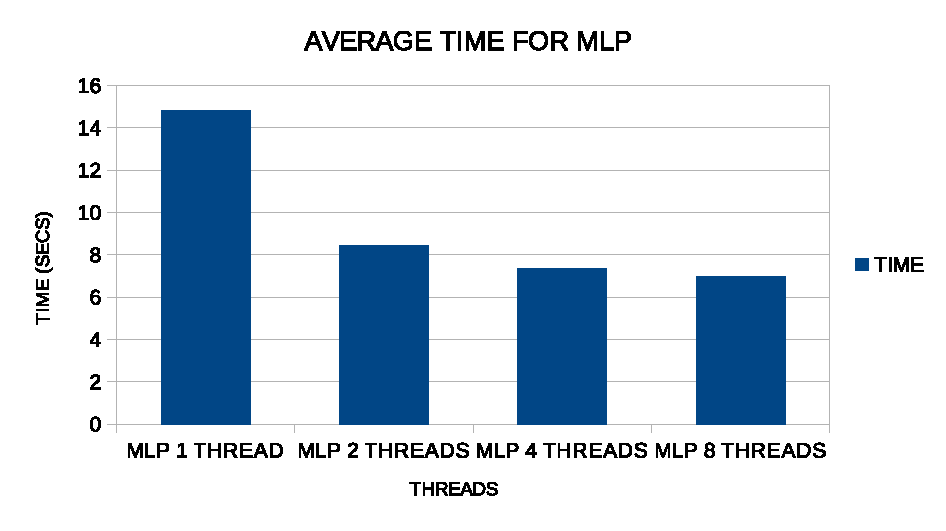
\includegraphics[scale=0.7]{timecomparison}
\end{figure}

\begin{figure}
\caption{Absolute error for the NLODE4 case.\label{fig:nlode4_error}}

\begin{centering}
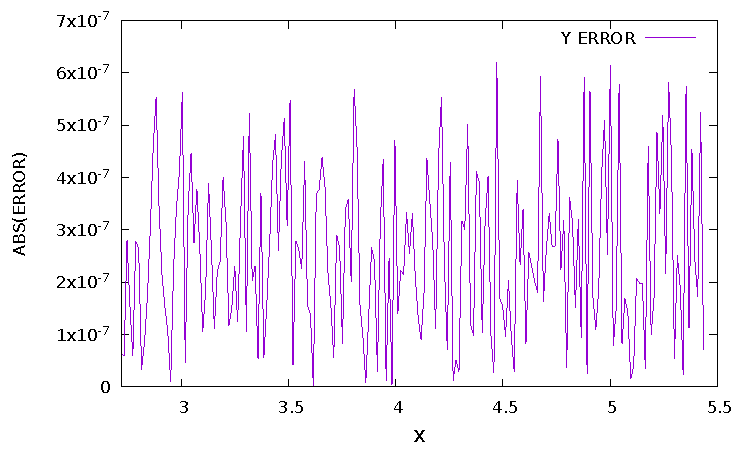
\includegraphics[scale=0.7]{nlode4_error}
\par\end{centering}
\end{figure}
\begin{figure}
\caption{Absolute error for the SODE2 test case.\label{fig:error_sode2}}

\begin{centering}
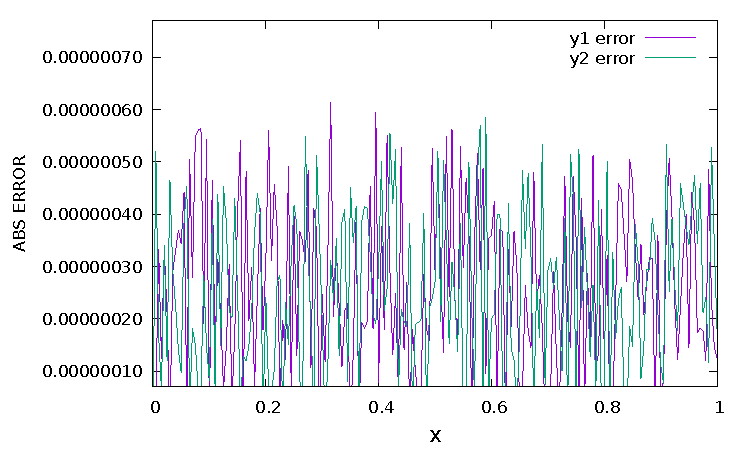
\includegraphics[scale=0.7]{sode2_error}
\par\end{centering}
\end{figure}


\subsection{Comparison with other methods}

In order to be able to understand the dynamics of the proposed methodology,
it was applied to a series of practical problems which are available
from the relevant website \url{ https://archimede.uniba.it/~testset/ }.
The obtained problems are the Hires problem, the Rober problem and
the Orego problem.

\subsubsection*{Hires problem }

The Hires problem was suggested by Sch�fer in 1975 \cite{de_hires}
and it describes how light is involved in morphogenesis. The problem
is defined as 
\[
\frac{dy}{dt}=f(y),\ y(0)=y_{0}
\]
where $t\in[0,321.8122]$ and the function $f(y)$ is the following
array of equations: 
\begin{eqnarray*}
f(y) & = & \left(\begin{array}{c}
-1.71y_{1}+0.43y_{2}+8.32y_{3}+0.0007\\
1.71y_{1}-8.75y_{2}\\
-10.03y_{3}+0.43y_{4}+0.035y_{5}\\
8.32y_{2}+1.71y_{3}-1.12y_{4}\\
-1.745y_{5}+0.43y_{6}+0.43y_{7}\\
-280y_{6}y_{8}+0.69y_{4}+1.71y_{5}-0.43y_{6}+0.69y_{7}\\
280y_{6}y_{8}-1.81y_{7}\\
-280y_{6}y_{8}+1.81y_{7}
\end{array}\right)
\end{eqnarray*}
The initial conditions of the system are: $y_{0}=\left(1,0,0,0,0,0,0,0.0057\right)$

\subsubsection*{Rober problem}

The Rober problem \cite{de_rober} describes the kinetics of an autocatalytic
reaction and the system of equations is: 
\begin{eqnarray*}
f(y) & = & \left(\begin{array}{c}
-0.04y_{1}+10^{4}y_{2}y_{3}\\
0.04y_{1}-10^{4}y_{2}y_{3}-3\times10^{7}y_{2}^{2}\\
3\times10^{7}y_{2}^{2}
\end{array}\right)
\end{eqnarray*}
with $t\in[0,10]$. The initial conditions are $y_{0}=\left(1,0,0\right)$.

\subsubsection*{Orego problem}

The Orego problem \cite{de_orego} describes the Oregonator model.
The problem is defined as 
\[
\frac{dy}{dt}=f(y),\ y(0)=y_{0}
\]
with $t\in[0,360]$ The function $f(y)$ is :
\begin{eqnarray*}
f(y) & = & \left(\begin{array}{c}
s\left(y_{2}-y_{1}y_{2}+y_{1}-qy_{1}^{2}\right)\\
\frac{1}{s}\left(-y_{2}-y_{1}y_{2}+y_{3}\right)\\
w\left(y_{1}-y_{3}\right)
\end{array}\right)
\end{eqnarray*}
with $y_{0}=\left(1,2,3\right)$ and $s=77.27,\ w=0.161,\ q=8.375\times10^{-6}$. 

The proposed method with the artificial neural network as model was
applied on the above practical problems. The experimental results
are compared against MEBDF \cite{de_memb} and are listed in the Table
\ref{tab:Comparison-with-MEMDB}. 

\begin{table}
\caption{Comparison with MEMDB method on some real world problems.\label{tab:Comparison-with-MEMDB}}

\centering{}%
\begin{tabular}{|c|c|c|c|}
\hline 
PROBLEM & MEBDF & MLP GEN & MLP PSO\tabularnewline
\hline 
\hline 
HIRES & $6.1\times10^{-1}$ & $7.6\times10^{-6}$ & $8.7\times10^{-6}$\tabularnewline
\hline 
OREGO & $1.2\times10^{-3}$ & $5.0\times10^{-11}$ & $1.5\times10^{-10}$\tabularnewline
\hline 
ROBER & $2.5\times10^{-2}$ & $2.66\times10^{-7}$ & $2.9\times10^{-7}$\tabularnewline
\hline 
\end{tabular}
\end{table}


\section{Conclusions \label{sec:Conclusions}}

In this text, the numerical solution of differential equations using
machine learning models was presented. These models were artificial
neural networks and RBF neural networks. The adjustment of the parameters
of these models to the initial conditions of the equations was done
using penalty factors. Finding the optimal parameters for these models
was done using two modified versions of well - known global optimization
techniques. One global optimization method used was the genetic algorithm
and the other modification was the particle swarm optimization. In
all experimental cases, the generalization error was extremely low
and, indeed, in some cases, the RBF network was shown to outperform
the artificial neural network.

Future extensions of the proposed methodology may include:
\begin{enumerate}
\item Incorporation of additional machine learning models, such as SVM models.
\item Usage of more efficient stopping rules. 
\item Parallelization of the whole process using modern programming techniques
such as MPI \cite{openmpi} or OpenMP \cite{openmp}.
\end{enumerate}
\begin{thebibliography}{10}
\bibitem{de_physics1}M. Raissi, G.E. Karniadakis, Hidden physics
models: Machine learning of nonlinear partial differential equations,
Journal of Computational Physics \textbf{357}, pp. 125-141, 2018.

\bibitem{de_physics2}T. Leli�vre, G. Stoltz, Partial differential
equations and stochastic methods in molecular dynamics. Acta Numerica
\textbf{25}, pp. 681-880, 2016.

\bibitem{de_chem1}G. Scholz, F. Scholz, First-order differential
equations in chemistry, ChemTexts \textbf{1}, 2015.

\bibitem{de_chem2}J.L. Padgett, Y. Geldiyev, S. Gautam, W. Peng,
Y. Mechref, A. Ibraguimov, Object classification in analytical chemistry
via data-driven discovery of partial differential equations. Comp
and Math Methods, 2021.

\bibitem{de_chem3}O. Owoyele, P. Pal, ChemNODE: A neural ordinary
differential equations framework for efficient chemical kinetic solvers,
Energy and AI \textbf{7}, 2022.

\bibitem{de_econ1}Z. Wang, X. Huang, H. Shen, Control of an uncertain
fractional order economic system via adaptive sliding mode, Neurocomputing
\textbf{83}, pp. 83-88, 2012.

\bibitem{de_econ2}Y. Achdou, F.J. Buera, J.M. Lasry, P.L. Lions,
B. Moll, Partial differential equation models in macroeconomicsPhil.
Trans. R. Soc. A. \textbf{372}, 2012.

\bibitem{de_bio1}K. Hattaf, N. Yousfi, Global stability for reaction--diffusion
equations in biology, Computers \& Mathematics with Applications \textbf{66},
pp. 1488-1497, 2013.

\bibitem{de_bio2}P. Getto, M. Waurick, A differential equation with
state-dependent delay from cell population biology, Journal of Differential
Equations \textbf{260}, pp. 6176-6200, 2016.

\bibitem{de_rk1}C.A. Kennedy, M.H. Carpenter, Higher-order additive
Runge--Kutta schemes for ordinary differential equations, Applied
Numerical Mathematics \textbf{136}, pp. 183-205, 2019.

\bibitem{de_rk2}H. Ranocha, D.I. Ketcheson, Relaxation Runge--Kutta
Methods for Hamiltonian Problems, J Sci Comput \textbf{84}, 17 2020.

\bibitem{de_rk3}J. Niegemann, R. Diehl, K. Busch, Efficient low-storage
Runge--Kutta schemes with optimized stability regions, Journal of
Computational Physics 231, pp. 364-372, 2012.

\bibitem{de_wave1}Y. Wang. Q. Fan, The second kind Chebyshev wavelet
method for solving fractional differential equations, Applied Mathematics
and Computation \textbf{218}, pp. 8592-8601, 2012.

\bibitem{de_wave2}M.H.Heydari, M.R.Hooshmandasl, F.Mohammadi, Legendre
wavelets method for solving fractional partial differential equations
with Dirichlet boundary conditions, Applied Mathematics and Computation
\textbf{234}, pp. 267-276, 2014.

\bibitem{de_wave3}B. Yuttanan, M. Razzaghi, Legendre wavelets approach
for numerical solutions of distributed order fractional differential
equations, Applied Mathematical Modelling \textbf{70}, pp. 350-364,
2019.

\bibitem{de_pred1}H. Kim, R. Sakthivel, Numerical solution of hybrid
fuzzy differential equations using improved predictor--corrector
method, Communications in Nonlinear Science and Numerical Simulation
\textbf{17}, pp. 3788-3794, 2012.

\bibitem{de_pred2}V. Daftardar-Gejji, Y. Sukale, S. Bhalekar, A new
predictor--corrector method for fractional differential equations,
Applied Mathematics and Computation \textbf{244}, pp. 158-182, 2014.

\bibitem{neural1}C. Bishop, Neural Networks for Pattern Recognition,
Oxford University Press, 1995.

\bibitem{neural2}G. Cybenko, Approximation by superpositions of a
sigmoidal function, Mathematics of Control Signals and Systems 2,
pp. 303-314, 1989.

\bibitem{de_nn1}I. E. Lagaris, A. Likas, D. I. Fotiadis, Artificial
neural networks for solving ordinary and partial differential equations,
IEEE Transactions on Neural Networks \textbf{9}, pp. 987-1000, 1998.

\bibitem{de_nn2}A. Malek, R.Shekari Beidokhti, Numerical solution
for high order differential equations using a hybrid neural network---Optimization
method, Applied Mathematics and Computation \textbf{183}, pp. 260-271,
2006.

\bibitem{de_nn3}W. Zhang, W. Cai, FBSDE based neural network algorithms
for high-dimensional quasilinear parabolic PDEs, Journal of Computational
Physics \textbf{470}, 2022.

\bibitem{de_finite1}P. Frauenfelder, C. Schwab, R.A. Todor, Finite
elements for elliptic problems with stochastic coefficients, Computer
Methods in Applied Mechanics and Engineering \textbf{194}, pp. 205-228,
2005.

\bibitem{de_finite2}P. Houston, E. S�li, A note on the design of
hp-adaptive finite element methods for elliptic partial differential
equations, Computer Methods in Applied Mechanics and Engineering \textbf{194},
pp. 229-243, 2005.

\bibitem{de_semimplicit1}L.Q.Chen, J. Shen, Applications of semi-implicit
Fourier-spectral method to phase field equations, Computer Physics
Communications 108, pp. 147-158, 1998.

\bibitem{de_semiimplicit2}P. Fedoseev, D. Pesterev, A. Karimov, D.
Butusov, New Step Size Control Algorithm for Semi-Implicit Composition
ODE Solvers, Algorithms \textbf{15}, article number 275, 2022. 

\bibitem{de_semiexplicit}A. Tutueva, T. Karimov, D. Butusov, Semi-Implicit
and Semi-Explicit Adams-Bashforth-Moulton Methods, Mathematics 8,
Article number 780, 2020.

\bibitem{de_semipred1}C. Clancy, J.A. Pudykiewicz, A class of semi-implicit
predictor--corrector schemes for the time integration of atmospheric
models, Journal of Computational Physics \textbf{250}, pp. 665-684,
2013.

\bibitem{de_semipred2}A. Tutueva, D. Butusov, Stability Analysis
and Optimization of Semi-Explicit Predictor--Corrector Methods, Mathematics
\textbf{9}, Article number 2463, 2021.

\bibitem{ge_main}M. O'Neill, C. Ryan, Grammatical evolution, IEEE
Transactions on Evolutionary Computation \textbf{5}, pp. 349-358,
2001.

\bibitem{de_tsoulos}I.G. Tsoulos, I.E. Lagaris, Solving differential
equations with genetic programming. Genet Program Evolvable Mach \textbf{7},
pp. 33--54, 2006.

\bibitem{de_svm1}S. Mehrkanoon, T. Falck and J. A. K. Suykens, Approximate
Solutions to Ordinary Differential Equations Using Least Squares Support
Vector Machines, IEEE Transactions on Neural Networks and Learning
Systems \textbf{23}, pp. 1356-1367, 2012.

\bibitem{de_svm2}S. Mehrkanoon, J.A.K.Suykens, Learning solutions
to partial differential equations using LS-SVM, Neurocomputing \textbf{159},
pp. 105-116, 2015.

\bibitem{de_deep1}J. Sirignano, K. Spiliopoulos, DGM: A deep learning
algorithm for solving partial differential equations, Journal of Computational
Physics \textbf{375}, pp. 1339-1364, 2018.

\bibitem{de_deep2}M.Raissi, P.Perdikaris, G.E.Karniadakis, Physics-informed
neural networks: A deep learning framework for solving forward and
inverse problems involving nonlinear partial differential equations,
Journal of Computational Physics \textbf{378}, pp. 686-707, 2019.

\bibitem{de_nnc}I.G. Tsoulos, D. Gavrilis, E. Glavas, Solving differential
equations with constructed neural networks \textbf{72}, pp. 2385-2391,
2009.

\bibitem{RbfMain}J. Park and I. W. Sandberg, Universal Approximation
Using Radial-Basis-Function Networks, Neural Computation 3, pp. 246-257,
1991.

\bibitem{ga1}D. Goldberg, Genetic Algorithms in Search, Optimization
and Machine Learning, Addison-Wesley Publishing Company, Reading,
Massachussets, 1989.

\bibitem{ga2}Z. Michaelewicz, Genetic Algorithms + Data Structures
= Evolution Programs. Springer - Verlag, Berlin, 1996.

\bibitem{ga3}S.A. Grady, M.Y. Hussaini, M.M. Abdullah, Placement
of wind turbines using genetic algorithms, Renewable Energy \textbf{30},
pp. 259-270, 2005.

\bibitem{pso1}J. Kennedy, R.C. Eberhart, The particle swarm: social
adaptation in information processing systems, in: D. Corne, M. Dorigo
and F. Glover (eds.), New ideas in Optimization, McGraw-Hill, Cambridge,
UK, pp. 11-32, 1999.

\bibitem{pso2}F. Marini, B. Walczak, Particle swarm optimization
(PSO). A tutorial, Chemometrics and Intelligent Laboratory Systems
\textbf{149}, pp. 153-165, 2015.

\bibitem{gen_par1}E.Cant�-Paz, D.E.Goldberg, Efficient parallel genetic
algorithms: theory and practice, Computer Methods in Applied Mechanics
and Engineering \textbf{186}, pp. 221-238, 2000.

\bibitem{gen_par2}K. Wang,Z. Shen, A GPU-Based Parallel Genetic Algorithm
for Generating Daily Activity Plans, IEEE Transactions on Intelligent
Transportation Systems \textbf{13}, pp. 1474-1480, Sept. 2012.

\bibitem{gen_par3}D. Ke\v{c}o, A. Subasi, J. Kevric, Cloud computing-based
parallel genetic algorithm for gene selection in cancer classification,
Neural Comput \& Applic \textbf{30}, pp. 1601--1610, 2018.

\bibitem{nn_de_similar1}S. Effati, M. Pakdaman, Artificial neural
network approach for solving fuzzy differential equations, Information
Sciences \textbf{180,} pp. 1434-1457, 2010.

\bibitem{nn_de_similar2}M. Pakdaman, A. Ahmadian, S. Effati, S. Salahshour,
D. Baleanu, Solving differential equations of fractional order using
an optimization technique based on training artificial neural network,
Applied Mathematics and Computation \textbf{293,} pp. 81-95, 2017.

\bibitem{nn_de_similar3}M. R. Admon, N. Senu, A. Ahmadian, Z. A.
Majid, S. Salahshour, A new efficient algorithm based on feedforward
neural network for solving differential equations of fractional order,
Communications in Nonlinear Science and Numerical Simulation \textbf{117},
106968, 2023.

\bibitem{nnphysics1}P. Baldi, K. Cranmer, T. Faucett et al, Parameterized
neural networks for high-energy physics, Eur. Phys. J. C \textbf{76},
2016.

\bibitem{nnphysics2}J. J. Valdas and G. Bonham-Carter, Time dependent
neural network models for detecting changes of state in complex processes:
Applications in earth sciences and astronomy, Neural Networks \textbf{19},
pp. 196-207, 2006

\bibitem{nnphysics3}G. Carleo,M. Troyer, Solving the quantum many-body
problem with artificial neural networks, Science \textbf{355}, pp.
602-606, 2017.

\bibitem{nnchem1}Lin Shen, Jingheng Wu, and Weitao Yang, Multiscale
Quantum Mechanics/Molecular Mechanics Simulations with Neural Networks,
Journal of Chemical Theory and Computation \textbf{12}, pp. 4934-4946,
2016.

\bibitem{nnchem2}Sergei Manzhos, Richard Dawes, Tucker Carrington,
Neural network-based approaches for building high dimensional and
quantum dynamics-friendly potential energy surfaces, Int. J. Quantum
Chem. \textbf{115}, pp. 1012-1020, 2015.

\bibitem{nnchem3}Jennifer N. Wei, David Duvenaud, and Al�n Aspuru-Guzik,
Neural Networks for the Prediction of Organic Chemistry Reactions,
ACS Central Science \textbf{2}, pp. 725-732, 2016.

\bibitem{nnmed1}Igor I. Baskin, David Winkler and Igor V. Tetko,
A renaissance of neural networks in drug discovery, Expert Opinion
on Drug Discovery \textbf{11}, pp. 785-795, 2016.

\bibitem{nnmed2}Ronadl Bartzatt, Prediction of Novel Anti-Ebola Virus
Compounds Utilizing Artificial Neural Network (ANN), Chemistry Faculty
Publications \textbf{49}, pp. 16-34, 2018.

\bibitem{nnc}I.G. Tsoulos, D. Gavrilis, E. Glavas, Neural network
construction and training using grammatical evolution, Neurocomputing
\textbf{72}, pp. 269-277, 2008.

\bibitem{rbfphysics1}P. Teng, Machine-learning quantum mechanics:
Solving quantum mechanics problems using radial basis function networks,
Phys. Rev. E \textbf{98}, 033305, 2018.

\bibitem{rbfchemistry1}Chuanhao Wan and Peter de B. Harrington, Self-Configuring
Radial Basis Function Neural Networks for Chemical Pattern Recognition,
J. Chem. Inf. Comput. Sci. \textbf{39}, 1049--1056, 1999.

\bibitem{rbfmed1}Y.P. Wang, J.W. Dang, Q. Li and S. Li, Multimodal
medical image fusion using fuzzy radial basis function neural networks,
in 2007 International Conference on Wavelet Analysis and Pattern Recognition,
pp. 778-782, 2017.

\bibitem{gen_app1}R.L. Haupt, An introduction to genetic algorithms
for electromagnetics, Antennas and Propagation Magazine 37, pp. 7-15,
1995.

\bibitem{gen_app2}J.J. Grefenstette, R. Gopal, B. J. Rosmaita, D.
Van Gucht, Genetic Algorithms for the Traveling Salesman Problem,
In: Proceedings of the 1st International Conference on Genetic Algorithms,
pp. 160 - 168, Lawrence Erlbaum Associates, 1985.

\bibitem{gen_app3}D. A. Savic, G. A. Walters, Genetic Algorithms
for Least-Cost Design of Water Distribution Networks, Journal of Water
Resources Planning and Management 123, pp. 67-77, 1997.

\bibitem{pso_app1}H. Yoshida, K. Kawata, Y. Fukuyama, S. Takayama,
Y. Nakanishi, A particle swarm optimization for reactive power and
voltagecontrol considering voltage security assessment, IEEE Transactions
on Power Systems \textbf{15}, pp. 1232-1239, 2000.

\bibitem{pso_app2}J. Robinson, Y. Rahmat-Samii, Particle swarm optimization
in electromagnetics, IEEE Transactions on Antennas and Propagation
\textbf{52}, pp. 397- 407, 2004.

\bibitem{pso_app3}M. A. Abido, Optimal power flow using particle
swarm optimization, International Journal of Electrical Power \& Energy
Systems \textbf{24}, pp. 563-571, 2002.

\bibitem{pso_app4}Z.L. Gaing, Particle swarm optimization to solving
the economic dispatch considering the generator constraints, IEEE
Transactions on Power Systems \textbf{18}, pp. 1187-1195, 2003.

\bibitem{powell}M.J.D Powell, A Tolerant Algorithm for Linearly Constrained
Optimization Calculations, Mathematical Programming \textbf{45}, pp.
547-566, 1989. 

\bibitem{kaeloAli}P. Kaelo, M.M. Ali, Integrated crossover rules
in real coded genetic algorithms, European Journal of Operational
Research \textbf{176}, pp. 60-76, 2007.

\bibitem{de_hires}E. Sch�fer, A new approach to explain the \textquotedblleft high
irradiance responses\textquotedblright{} of photomorphogenesis on
the basis of phytochrome. J. Math. Biology \textbf{2}, pp. 41--56,
1975.

\bibitem{de_rober}H.H. Robertson, H.H. The Solution of a Set of Reaction
Rate Equations. In: Walsh, J., Ed., Numerical Analysis: An introduction,
Academic Press, Cambridge, Massachusetts, pp. 178-182, 1967.

\bibitem{de_orego}E. Hairer, G. Wanner, Solving Ordinary Di erential
Equations II: Sti and Di erential- algebraic Problems. Springer-Verlag,
second revised edition, 1996.

\bibitem{de_memb}.R. Cash, S. Considine, An MEBDF code for stiff
initial value problems, ACM Trans. Math. Software \textbf{18}, pp.
142-158, 1992.

\bibitem{openmpi}R. L. Graham, G. M. Shipman, B. W. Barrett, R. H.
Castain, G. Bosilca and A. Lumsdaine, \textquotedbl Open MPI: A High-Performance,
Heterogeneous MPI,\textquotedbl{} 2006 IEEE International Conference
on Cluster Computing, 2006, pp. 1-9.

\bibitem{openmp}L. Dagum, R. Menon, OpenMP: an industry standard
API for shared-memory programming, IEEE Computational Science and
Engineering \textbf{5}, pp. 46-55, 1998.

\end{thebibliography}

\end{document}
